\chapter{Technical Details}
\label{cha:TechnicalDetails}

This section provides an in-depth overview of the architecture, implementation, and key components of TRUST. It covers the cryptographic protocols used, system architecture, core libraries, and design decisions that ensure security and usability.

The application is built using Rust’s asynchronous runtime (\texttt{tokio}) and the  framework for networking is \texttt{tokio-tungstenite}, while the user interface is implemented with \texttt{ratatui}. X3DH and Double Ratchet were implemented using primitives provided by the \texttt{dalek-cryptography} library, and AES-GCM using primitives provided by the \texttt{aes\_gcm} library, ensuring end-to-end encryption for user messages.

% TODO bisogna aggiunere la parte di Double Ratchet

\section{Architecture}
\label{sec:Architecture}

The application follows a client-server architecture with some modifications to enhance flexibility. By leveraging \textbf{WebSockets}, which provide bidirectional TCP communication, both the client and server can initiate requests. This approach simplifies development by enabling real-time message exchange without requiring traditional request-response cycles, making the system more efficient and responsive.


\subsection{Architecture overview}
\label{subsec:ArchitectureOverview}
From Server-side, incoming connections from clients are handled leveraging different threads, each responsible for managing a specific client connection.
Upon start up, the server call the \texttt{listen} method which is responsible for accepting incoming connections and spawning a new thread, named \texttt{acceptor}, for each connection. Each thread is responsible for handling the communication with a specific client, allowing the server to manage multiple clients simultaneously. The \texttt{acceptor} thread is responsible for initializing and managing the connection, to doing so, it spaws two additional threads, named \texttt{task\_receiver} and \texttt{task\_sender}. The \texttt{task\_receiver} thread is responsible for listening for incoming requests from the client and send responses back, while the \texttt{task\_sender} thread is responsible for forwarding messages to the client (see fig. \ref{fig:architecture-overview}).
The client, on the other hand, is designed to be a terminal-based user interface (TUI) application that interacts with the server. It consists of a main process that manages the user interface and sends requests to the server, a separate thread for listening to incoming responses or messages and forwarding them to the TUI, ultimetly the TUI levarages on a \texttt{tokio} task that listens for incoming messages on a \texttt{mpsc channel} and invokes the appropriate handler to process the message and render it in the user interface (see fig. \ref{fig:client-architecture-overview}).\\

To better understand the application's functionality, we outline four key scenarios that define its core operations:

\begin{enumerate}
    \item \textbf{Establishment of a Secure Connection}: The client and server perform a handshake to initiate a secure, encrypted communication channel.
    \item \textbf{User Registration}: New users send their public keys and register with the server while ensuring their identity remains protected.
    \item \textbf{Adding a Friend}: Users exchange public keys and establish a secure communication channel for encrypted messaging.
    \item \textbf{Sending Messages}: Messages are encrypted, transmitted over WebSockets, and decrypted on the recipient’s side, ensuring end-to-end security.
\end{enumerate}

Each of these steps plays a crucial role in maintaining the privacy and integrity of user interactions. The following sections describe these scenarios in detail.

\subsection{Establishment of a Secure Connection}
\label{subsec:EstablishmentOfASecureConnection}

The secure connection process begins with a standard \textbf{WebSocket handshake} (Figure \ref{fig:websocket-handshake}) between the client and server. Once the bidirectional channel is established, the client transmits its \textbf{Pre-Key Bundle}, which the server processes to:

\begin{itemize}
    \item Derive the shared key used to encrypt communications.
    \item Generate the \textbf{Server Initial Message (SIM)}, which is then sent back to the client.
\end{itemize}

\begin{figure}[!ht]
    \centering
    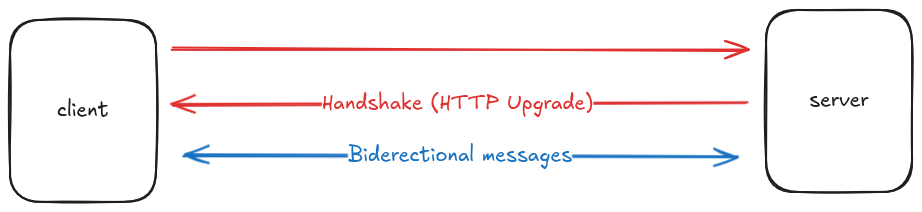
\includegraphics[width=0.8\linewidth]{imgs/Websocket.png}
    \caption{WebSocket Handshake}
    \label{fig:websocket-handshake}
\end{figure}

Upon receiving the SIM, the client verifies the server’s identity by comparing the known \textbf{server public identity key} with the one provided in the message. This prevents \textbf{Man-in-the-Middle (MitM) attacks}. If authentication is successful, the client processes the SIM and derives the shared key. From this point forward, all communication between the client and server will be encrypted.

\begin{figure}[!ht]
    \centering
    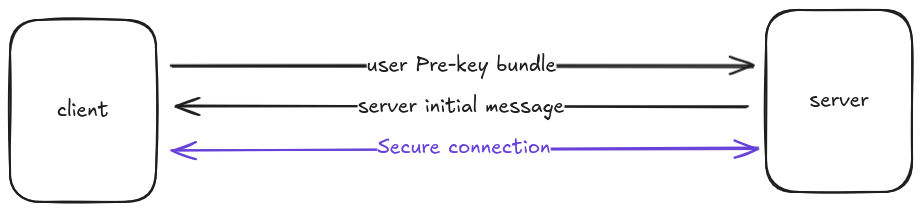
\includegraphics[width=0.8\linewidth]{imgs/secure-connection.png}
    \caption{Secure connection establishment}
    \label{fig:secure-connection}
\end{figure}

\subsection{User Registration}
\label{subsec:UserRegistration}

Once a secure connection with the server is established, the user can register by choosing a \textbf{username} and sending a \textbf{registration request} to the server. The server then verifies whether the chosen username is unique.

\begin{itemize}
    \item If the username is \textbf{available}, the server sends a \textbf{confirmation response} to the client.
    \item If the username is \textbf{already taken}, the server responds with a \texttt{"Conflict"} status code and the message \texttt{"User Already Exists"}, prompting the user to choose a different username.
\end{itemize}

\begin{lstlisting}[language=json, caption= Example of a Registration request]
{
    "action":"register",
    "username":"xyz",
    "bundle:"dGhpcyBpcyB0aGUgdXNlciBwcmVrZXkgYnVuZGxGluIGJ2U2NA=="
}
\end{lstlisting}

\subsection{Adding a Friend}
\label{subsec:AddingAFriend}

Once the user is registered in the system, they can add a new friend by submitting a \textbf{get user pre-key bundle request} to the server, specifying the username of the desired contact. The server then checks whether the requested user is registered in the application.

\begin{itemize}
    \item If the user \textbf{exists}, the server responds with the requested user's \textbf{Pre-Key Bundle}.
    \item If the user \textbf{is not found}, the server returns a \texttt{"UserNotFound"} error response with \texttt{status code 404}.
\end{itemize}

\subsection{Sending Messages}
\label{subsec:SendingMessages}

% TODO bisogna aggiunere la parte di Double Ratchet

Upon receiving the requested user's \textbf{Pre-Key Bundle}, the user derives the \textbf{shared key} and generates the \textbf{initial message}. The user then sends a \texttt{send\_message} request to the recipient, embedding the initial message in the \texttt{"text"} field. The request follows the JSON format below:

\begin{lstlisting}[language=json, caption={Initial Message Request Format}]
{
  "action": "send_message",
  "msg_type": "initial_message",
  "to": "alice",
  "from": "bob",
  "text": "dGhpcyBpcyB0aGXNlciBpbml0aWFsIG1lc3NhZ2UgaW4gYmFzZTY0",
  "timestamp": "2025-02-06T14:21:21+00:00"
}
\end{lstlisting}

The user who will receive the initial message will derive the shared key and then add the sender as a contact in their contacts list.

\section{Implementation}
\label{sec:Implementation}

This section will provide a comprehensive explanation of the implementation of each key component of the application. Each aspect of the application, from the underlying security mechanisms to the user-facing interface, is discussed in detail to give a clear understanding of the technical choices and how they come together to ensure a seamless and secure user experience.

\subsection{Key Generation for X3DH}
\label{subsec:KeyGeneration}

The function responsible for generating \textbf{Pre-Key Bundles} is \texttt{generate\_prekey\_bundle()}. This function creates the \textbf{Private Identity Key}, \textbf{Private Signed Pre-Key}, and their corresponding \textbf{Public Keys}. Additionally, it returns the \textbf{Pre-Key Bundle} along with the \textbf{private keys} required for secure communication.

To prevent \textbf{replay attacks}, \textbf{One-Time Pre-Keys (OTPKs)} are incorporated into the key generation process. For this purpose, a specialized function, \\ \texttt{generate\_prekey\_bundle\_with\_otpk()}, is introduced. This function takes as input the number of \textbf{one-time pre-keys} to generate and returns a tuple containing:
\begin{itemize}
    \item The \textbf{Pre-Key Bundle},
    \item The \textbf{Private Identity Key},
    \item The \textbf{Private Signed Pre-Key},
    \item A vector of \textbf{private One-Time Pre-Keys}.
\end{itemize}

This approach ensures that each session can maintain \textbf{forward secrecy} while mitigating potential security risks such as \textbf{key reuse and replay attacks}.

\subsection{Pre-Key Bundle Processing}
\label{subsec:Pre-KeyBundleProcessing}

The function responsible for processing \textbf{Pre-Key Bundles} is \texttt{process\_prekey\_bundle()}, which takes as input the received bundle and the receiver's \textbf{Private Identity Key}.

The function first verifies the signature contained in the bundle to ensure its authenticity. After validation, it performs the \textbf{X3DH (Extended Triple Diffie-Hellman) key agreement protocol} to derive the shared secret. This is done by passing the secret obtained from the three Diffie-Hellman exchanges through a \textbf{Key Derivation Function (KDF)} to generate the final 32-byte shared key.  

Once the shared key is established, an \textbf{Initial Message (IM)} is generated, containing the following components:  

\begin{itemize}  
    \item The receiver's \textbf{Public Identity Key};  
    \item The receiver's \textbf{Public Ephemeral Key};  
    \item The sender's \textbf{Public Signed Pre-Key hash} (extracted from the bundle);  
    \item The sender's \textbf{Public One-Time Pre-Key (OTPK) hash};  
    \item \textbf{Associated Data}, which includes the Public Identity Keys of both the sender and receiver.  
\end{itemize}  

The function then returns the shared key and the initial message.

\subsection{Initial Message Processing}
\label{subsec:InitialMessageProcessing}

The functions responsible for processing the \textbf{Initial Message} are respectively \\ \texttt{process\_server\_initial\_message()} and \texttt{process\_initial\_message()}. These two functions are equivalent, except that the former additionally verifies whether the \textbf{Server's Public Identity Key} provided as input matches the one included in the Initial Message.  

Both functions take as input the received Initial Message, the receiver's \textbf{Private Identity Key}, \textbf{Private Signed Key}, and \textbf{Private One-Time Pre-Key (OTPK)}. They compute the three Diffie-Hellman (3DH) secrets and pass the resulting value through a \textbf{Key Derivation Function (KDF)} to derive the 32-byte shared key. Finally, they return the computed shared key.  

\subsection{AES Encryption}
\label{subsec:AESEncryption}

The function responsible for AES encryption is \texttt{encrypt()}. This function takes as input the encryption key, the data to be encrypted, and the \textbf{Associated Data (AD)}.

First, it generates a nonce using the Cryptographically Secure Pseudo Random Number Generator (CSPRNG) provided by the \texttt{rand} crate in Rust (OsRng). Then, it constructs the payload and performs AES-GCM encryption. Finally, it concatenates the nonce, the associated data, and the ciphertext before returning the result as a \textbf{Base64-encoded string}.

\subsection{AES Decryption}
\label{subsec:AESDecryption}

The function responsible for AES decryption is \texttt{decrypt()}. It takes as input the decryption key, the cipher text to be decrypted, and the \textbf{Associated Data (AD)} and the \textbf{Nonce}.

This function checks for integrity and then performs the inverse operation of the encryption process if the message has not been tampered with. Finally, it returns the decrypted data as a \textbf{byte vector}.


\subsection{Server}
\label{subsec:Server}
The server implementation is built on an asynchronous runtime provided by the \texttt{tokio} library in Rust. This library enables the server to perform non-blocking asynchronous operations, improving both flexibility and performance.  

Each new connection is handled by a separate Tokio task, allowing the server to efficiently manage multiple concurrent connections. For each \textbf{Connection task}, two additional Tokio tasks are generated:

\begin{itemize}
    \item the first task (\texttt{task\_receiver}) continuously listen for incoming requests;
    \item the second task (\texttt{task\_sender}) forwards messages to the client;
\end{itemize}

\subsubsection{Task Receiver}
\label{subsec:TaskReceiver}

This task continuously listens for incoming requests on the WebSocket connection from the client. It exposes four API endpoints:

\begin{itemize}
    \item \texttt{establish\_connection}: Used to establish a secure connection between the client and the server. This API endpoint is handled by the function \\
    \texttt{handle\_establish\_connection()}, which first verifies whether the Pre-Key bundle is correctly formatted. If the verification is successful, the function calls  \\
    \texttt{process\_key\_bundle()} to generate the shared secret; otherwise, it returns an error. Once the shared secret is derived, it is stored in a shared variable called \texttt{session}, allowing both tasks to access it. This endpoint is only accessible if no shared secret exists, meaning that a secure connection has not yet been established.

    \item \texttt{register}: Accessible once the secure connection is established, allowing the client to register within the application. This API endpoint is handled by the function \texttt{handle\_registration\_request()}, which first performs the necessary username validation (ensuring it is alphanumeric and not already in use). It then verifies whether the Pre-Key bundle is well-formed. If all checks pass, the user is registered in the system and it sends back a confirmation response.

    \item \texttt{get\_user\_bundle}: Accessible after the secure connection is established, enabling the client to retrieve a user's key bundle. This API endpoint is handled by the function \texttt{handle\_get\_bundle\_request()}, which verifies whether the requested user is registered in the system. If the user exists, the function generates a response containing the corresponding key bundle; otherwise, it returns a \texttt{User Not Found} error.

    \item \texttt{send\_message}: Available once the secure connection is established, allowing the client to exchange messages with other users. This API endpoint is handled directly by the task. It first checks whether the recipient is registered (and thus connected) to the system. If the recipient is online, the task forwards the message to the recipient's sender task, which then delivers it to the recipient's client.
\end{itemize}

All API requests received after the secure connection is established are decrypted upon arrival, and all responses are encrypted before being sent to the client. 

\subsubsection{Task Sender}
\label{subsec:TaskSender}

The Task Sender is responsible for message forwarding. It continuously listens on a \texttt{mpsc channel} for incoming messages. Upon receiving a message, it encrypts the content using the session key shared between the recipient client and the server, ensuring secure communication. Once the message is encrypted, it forwards the encrypted message to the recipient.

The content of messages is encrypted using the shared key between the two clients. The \texttt{send\_message} request undergoes two layers of encryption: first, the message text is encrypted with the shared key between the clients, and then the entire request is encrypted using the shared key between the client and the server, ensuring end-to-end security.

%put image here
\begin{figure}
  \centering
  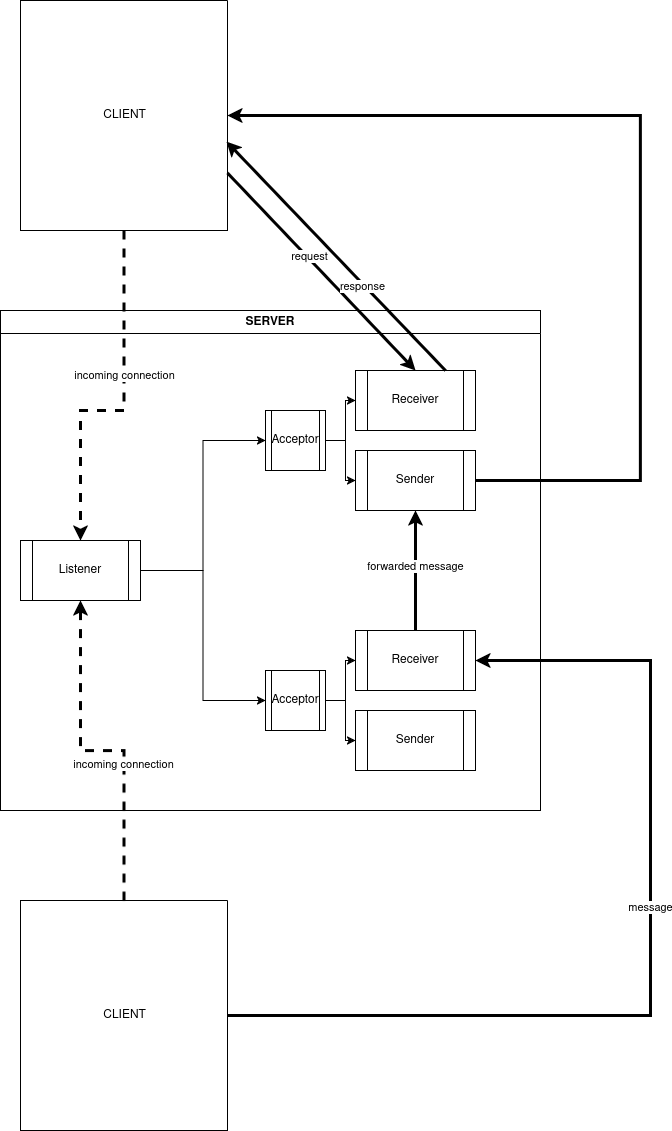
\includegraphics[width=0.8\linewidth]{imgs/server-arch.png}
  \caption{Server Architecture Overview}
  \label{fig:architecture-overview}
\end{figure}



\begin{figure}
  \centering
  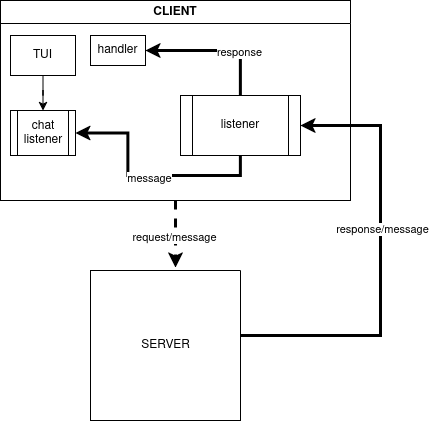
\includegraphics[width=0.8\linewidth]{imgs/client-arch.png}
  \caption{Client Architecture Overview}
  \label{fig:client-architecture-overview}
\end{figure}

\subsection{Client \& TUI}
\label{subsec:ClientTUI}

The client backend also utilizes \texttt{tokio} for asynchronous runtime. When a new client is created (i.e., when the TUI program is started), it attempts to establish a secure connection with the server. If successful, it spawns a Tokio listener task, which continuously listens for incoming responses or new messages.  

To manage the correlation between requests and responses, we introduced a struct called \texttt{RequestWrapper}. This struct contains two fields: \texttt{request\_uuid}, which uniquely identifies the request, and \texttt{body}, which holds the actual request to be sent to the server. When the server responds, it includes the same \texttt{request\_uuid} in the \texttt{ResponseWrapper}, allowing the client to match each response to its corresponding request.  

Chat messages, on the other hand, are handled as regular \texttt{send\_message} requests. When the client receives a message, it forwards it to a task running in the TUI binary, which listens for incoming messages on a \texttt{mpsc channel}. This task then invokes the appropriate handler to process the message and render it in the user interface.
\newpage
\section{Code Structure}
\label{sec:CodeStructure}

%TODO la struttura e' cambiata aggiungendo la perte di dr

The codebase is organized into five separate Cargo projects, each serving a distinct purpose:

\begin{itemize}
    \item \textbf{Protocol}: A library that implements the cryptographic protocols used in the system, including X3DH and AES-GCM.
    \item \textbf{Common}: A shared library providing utility functions used by both the client and server.
    \item \textbf{Server}: Contains the server binary along with all necessary utility functions for server-side operations.
    \item \textbf{Client}: A library that facilitates client interactions with the server.
    \item \textbf{Tui}: Includes the TUI application binary, along with all files required for the user interface and front-end logic.
\end{itemize}

\section{Dependencies}
\label{sec:Dependecies}

% TODO non sono sicuro se dr abbia aggiunto altre dependencies ma se si bisogna aggiungerle

The implementation of \textbf{TRUST} application relies on several external Rust crates that provide critical functionalities such as asynchronous networking, cryptographic operations, and terminal user interface (TUI) rendering. All dependencies used in this project are well-known, actively maintained, and considered de facto standards in their respective domains, ensuring reliability, security, and long-term support. Below is an overview of the main dependencies.   

\subsection{Networking and Asynchronous Execution}
\label{subsec:NetworkingAndAsynchronousExecution}

The list of dependencies used for the asynchronous execution is:

\begin{itemize}
  \item \textbf{\texttt{tokio} (1.42.0)}: Provides the asynchronous runtime used throughout the application to handle concurrent tasks efficiently, enabling non-blocking communication between clients and the server.
  \item \textbf{\texttt{tokio-tungstenite} (0.26.1)}: A WebSocket library that integrates with Tokio, allowing real-time, bidirectional communication over WebSockets.
  \item \textbf{\texttt{futures} (0.3.31) \& \texttt{futures-util} (0.3.31)}: Provide abstractions for asynchronous programming, including streams and futures for handling asynchronous events.
  \item \textbf{\texttt{tokio-stream} (0.1.17)}: Enhances stream handling within Tokio-based applications, making it easier to process asynchronous data flows.
\end{itemize}

\subsection{Cryptography and Secure Communication}
\label{subsec:CryptographyAndSecureCommunication}

The list of dependencies used for cryptographic purposes on the other hand is:

\begin{itemize}
  \item \textbf{\texttt{aes} (0.8.4) \& \texttt{aes-gcm} (0.10.3)}: Provide authenticated encryption for securing messages using the AES-GCM encryption scheme.
  \item \textbf{\texttt{rand} (0.8.5)}: A cryptographically secure random number generator, essential for generating nonces securely.
  \item \textbf{\texttt{ed25519-dalek} (2.1.1)}: Implements the Ed25519 signature scheme, ensuring authentication and integrity of messages.
  \item \textbf{\texttt{x25519-dalek} (2.0.1)}: Used for implementing the X3DH key exchange protocol, allowing secure key agreement between clients.
  \item \textbf{\texttt{curve25519-dalek} (4.1.3)}: Provides elliptic curve operations, specifically for Diffie-Hellman key exchange and digital signatures.
  \item \textbf{\texttt{sha2} (0.10.8)}: Implements the SHA-2 family of cryptographic hash functions, ensuring data integrity and secure hashing of credentials.
  \item \textbf{\texttt{hkdf} (0.12.4)}: Implements the HMAC-based Key Derivation Function (HKDF) used to derive cryptographic keys securely.
  \item \textbf{\texttt{zeroize} (1.8.1)}: Ensures that sensitive cryptographic data is securely erased from memory when no longer needed.
\end{itemize}

\subsection{Data Serialization and Parsing}  
\label{subsec:DataSerializatinAndParsin}

The dependencies used for data serialization is:

\begin{itemize}
  \item \textbf{\texttt{serde} (1.0.216) \& \texttt{serde\_json} (1.0.137)}: Used for serializing and deserializing data exchanged between the client and server.
  \item \textbf{\texttt{base64} (0.22.1)}: Handles encoding and decoding of binary data, particularly for securely transmitting encrypted messages.
\end{itemize}

\subsection{Terminal User Interface (TUI)}  
\label{subsed:TerminalUserInterfaceTUI}

For the TUI we chose the following dependencies:

\begin{itemize}
  \item \textbf{\texttt{ratatui} (0.29.0)}: A Rust TUI library used to create the command-line interface for the chat application.
  \item \textbf{\texttt{crossterm} (0.28.1)}: Provides cross-platform support for handling terminal input and output, including event handling and text rendering.
\end{itemize}

\subsection{Utilities}
\label{subsec:Utilities}

Finally some extra packeges chosen for extra utilities are:

\begin{itemize}
  \item \textbf{\texttt{uuid} (1.11.0)}: Used for generating unique request identifiers, allowing the system to match server responses with client requests.
  \item \textbf{\texttt{arrayref} (0.3.9)}: Provides utilities for working with fixed-size arrays, useful in cryptographic operations.
\end{itemize}

These dependencies collectively enable our application to provide secure, efficient, and user-friendly encrypted messaging.  
